% Options for packages loaded elsewhere
\PassOptionsToPackage{unicode}{hyperref}
\PassOptionsToPackage{hyphens}{url}
\PassOptionsToPackage{dvipsnames,svgnames,x11names}{xcolor}
%
\documentclass[
  letterpaper,
  DIV=11,
  numbers=noendperiod]{scrreprt}

\usepackage{amsmath,amssymb}
\usepackage{lmodern}
\usepackage{iftex}
\ifPDFTeX
  \usepackage[T1]{fontenc}
  \usepackage[utf8]{inputenc}
  \usepackage{textcomp} % provide euro and other symbols
\else % if luatex or xetex
  \usepackage{unicode-math}
  \defaultfontfeatures{Scale=MatchLowercase}
  \defaultfontfeatures[\rmfamily]{Ligatures=TeX,Scale=1}
\fi
% Use upquote if available, for straight quotes in verbatim environments
\IfFileExists{upquote.sty}{\usepackage{upquote}}{}
\IfFileExists{microtype.sty}{% use microtype if available
  \usepackage[]{microtype}
  \UseMicrotypeSet[protrusion]{basicmath} % disable protrusion for tt fonts
}{}
\makeatletter
\@ifundefined{KOMAClassName}{% if non-KOMA class
  \IfFileExists{parskip.sty}{%
    \usepackage{parskip}
  }{% else
    \setlength{\parindent}{0pt}
    \setlength{\parskip}{6pt plus 2pt minus 1pt}}
}{% if KOMA class
  \KOMAoptions{parskip=half}}
\makeatother
\usepackage{xcolor}
\setlength{\emergencystretch}{3em} % prevent overfull lines
\setcounter{secnumdepth}{5}
% Make \paragraph and \subparagraph free-standing
\ifx\paragraph\undefined\else
  \let\oldparagraph\paragraph
  \renewcommand{\paragraph}[1]{\oldparagraph{#1}\mbox{}}
\fi
\ifx\subparagraph\undefined\else
  \let\oldsubparagraph\subparagraph
  \renewcommand{\subparagraph}[1]{\oldsubparagraph{#1}\mbox{}}
\fi


\providecommand{\tightlist}{%
  \setlength{\itemsep}{0pt}\setlength{\parskip}{0pt}}\usepackage{longtable,booktabs,array}
\usepackage{calc} % for calculating minipage widths
% Correct order of tables after \paragraph or \subparagraph
\usepackage{etoolbox}
\makeatletter
\patchcmd\longtable{\par}{\if@noskipsec\mbox{}\fi\par}{}{}
\makeatother
% Allow footnotes in longtable head/foot
\IfFileExists{footnotehyper.sty}{\usepackage{footnotehyper}}{\usepackage{footnote}}
\makesavenoteenv{longtable}
\usepackage{graphicx}
\makeatletter
\def\maxwidth{\ifdim\Gin@nat@width>\linewidth\linewidth\else\Gin@nat@width\fi}
\def\maxheight{\ifdim\Gin@nat@height>\textheight\textheight\else\Gin@nat@height\fi}
\makeatother
% Scale images if necessary, so that they will not overflow the page
% margins by default, and it is still possible to overwrite the defaults
% using explicit options in \includegraphics[width, height, ...]{}
\setkeys{Gin}{width=\maxwidth,height=\maxheight,keepaspectratio}
% Set default figure placement to htbp
\makeatletter
\def\fps@figure{htbp}
\makeatother

\KOMAoption{captions}{tableheading}
\makeatletter
\@ifpackageloaded{tcolorbox}{}{\usepackage[many]{tcolorbox}}
\@ifpackageloaded{fontawesome5}{}{\usepackage{fontawesome5}}
\definecolor{quarto-callout-color}{HTML}{909090}
\definecolor{quarto-callout-note-color}{HTML}{0758E5}
\definecolor{quarto-callout-important-color}{HTML}{CC1914}
\definecolor{quarto-callout-warning-color}{HTML}{EB9113}
\definecolor{quarto-callout-tip-color}{HTML}{00A047}
\definecolor{quarto-callout-caution-color}{HTML}{FC5300}
\definecolor{quarto-callout-color-frame}{HTML}{acacac}
\definecolor{quarto-callout-note-color-frame}{HTML}{4582ec}
\definecolor{quarto-callout-important-color-frame}{HTML}{d9534f}
\definecolor{quarto-callout-warning-color-frame}{HTML}{f0ad4e}
\definecolor{quarto-callout-tip-color-frame}{HTML}{02b875}
\definecolor{quarto-callout-caution-color-frame}{HTML}{fd7e14}
\makeatother
\makeatletter
\makeatother
\makeatletter
\@ifpackageloaded{bookmark}{}{\usepackage{bookmark}}
\makeatother
\makeatletter
\@ifpackageloaded{caption}{}{\usepackage{caption}}
\AtBeginDocument{%
\ifdefined\contentsname
  \renewcommand*\contentsname{Tabla de contenidos}
\else
  \newcommand\contentsname{Tabla de contenidos}
\fi
\ifdefined\listfigurename
  \renewcommand*\listfigurename{Listado de Figuras}
\else
  \newcommand\listfigurename{Listado de Figuras}
\fi
\ifdefined\listtablename
  \renewcommand*\listtablename{Listado de Tablas}
\else
  \newcommand\listtablename{Listado de Tablas}
\fi
\ifdefined\figurename
  \renewcommand*\figurename{Figura}
\else
  \newcommand\figurename{Figura}
\fi
\ifdefined\tablename
  \renewcommand*\tablename{Tabla}
\else
  \newcommand\tablename{Tabla}
\fi
}
\@ifpackageloaded{float}{}{\usepackage{float}}
\floatstyle{ruled}
\@ifundefined{c@chapter}{\newfloat{codelisting}{h}{lop}}{\newfloat{codelisting}{h}{lop}[chapter]}
\floatname{codelisting}{Listado}
\newcommand*\listoflistings{\listof{codelisting}{Listado de Listados}}
\makeatother
\makeatletter
\@ifpackageloaded{caption}{}{\usepackage{caption}}
\@ifpackageloaded{subcaption}{}{\usepackage{subcaption}}
\makeatother
\makeatletter
\@ifpackageloaded{tcolorbox}{}{\usepackage[many]{tcolorbox}}
\makeatother
\makeatletter
\@ifundefined{shadecolor}{\definecolor{shadecolor}{rgb}{.97, .97, .97}}
\makeatother
\makeatletter
\makeatother
\ifLuaTeX
\usepackage[bidi=basic]{babel}
\else
\usepackage[bidi=default]{babel}
\fi
\babelprovide[main,import]{spanish}
% get rid of language-specific shorthands (see #6817):
\let\LanguageShortHands\languageshorthands
\def\languageshorthands#1{}
\ifLuaTeX
  \usepackage{selnolig}  % disable illegal ligatures
\fi
\IfFileExists{bookmark.sty}{\usepackage{bookmark}}{\usepackage{hyperref}}
\IfFileExists{xurl.sty}{\usepackage{xurl}}{} % add URL line breaks if available
\urlstyle{same} % disable monospaced font for URLs
\hypersetup{
  pdftitle={Certificación European Financial Advisor - EFA™     Asociación Europea de Planificación Financiera - EFPA™},
  pdfauthor={Profesor Alberto Bernat   Máster en Dirección y Planificación Financiera   Universidad Europea Miguel de Cervantes   Economista (Colegiado nº. 3.685)   Asesor Financiero (EFA nº. 14.672)},
  pdflang={es},
  colorlinks=true,
  linkcolor={blue},
  filecolor={Maroon},
  citecolor={Blue},
  urlcolor={Blue},
  pdfcreator={LaTeX via pandoc}}

\title{Certificación European Financial Advisor - EFA™ Asociación
Europea de Planificación Financiera - EFPA™}
\usepackage{etoolbox}
\makeatletter
\providecommand{\subtitle}[1]{% add subtitle to \maketitle
  \apptocmd{\@title}{\par {\large #1 \par}}{}{}
}
\makeatother
\subtitle{ \textbf{Ejercicios y exámenes resueltos}}
\author{\href{https://www.linkedin.com/in/albertobernat/}{\emph{\textbf{Profesor
Alberto Bernat}}} Máster en Dirección y Planificación Financiera
Universidad Europea Miguel de Cervantes Economista (Colegiado nº. 3.685)
Asesor Financiero (EFA nº. 14.672)}
\date{20/2/23}

\begin{document}
\maketitle
\ifdefined\Shaded\renewenvironment{Shaded}{\begin{tcolorbox}[boxrule=0pt, interior hidden, borderline west={3pt}{0pt}{shadecolor}, enhanced, breakable, sharp corners, frame hidden]}{\end{tcolorbox}}\fi

\renewcommand*\contentsname{Tabla de contenidos}
{
\hypersetup{linkcolor=}
\setcounter{tocdepth}{2}
\tableofcontents
}
\bookmarksetup{startatroot}

\hypertarget{introducciuxf3n}{%
\chapter*{\texorpdfstring{\textsc{INTRODUCCIÓN}}{INTRODUCCIÓN}}\label{introducciuxf3n}}
\addcontentsline{toc}{chapter}{\textsc{INTRODUCCIÓN}}

\markboth{\textsc{INTRODUCCIÓN}}{\textsc{INTRODUCCIÓN}}

Desde que en 2017 la
\href{https://www.cnmv.es/portal/home.aspx}{Comisión Nacional del
Mercado de Valores (CNMV)} publicase la relación de
\href{http://cnmv.es/Docportal/Legislacion/Titulos/ListadoTitulos.pdf}{títulos
asociados a distintas organizaciones y universidades que acreditan el
cumplimiento de los requisitos recogidos en la Guía Técnica, en atención
a lo que establece MiFID II} las entidades y profesionales
pertenecientes al sector financiero español, se encuentran en la
obligación de tener que certificar la posesión de alguno de estos
títulos frente a la CNMV.

Estos títulos \textbf{acreditarán al personal que trabaja en el sector
su capacidad para asesorar e informar} o, \textbf{solamente la capacidad
para poder realizar labores de información} en materia de inversión.
Esta capacidad se establece en función del \textbf{número de horas de
formación y también en función los contenidos que se comprenden dentro
de los cursos} para la obtención de los respectivos títulos.

En otras palabras, podemos decir que se trata de \textbf{demostrar
frente al regulador estatal} que el personal que informa o asesora sobre
servicios de inversión posee los conocimientos y competencias
necesarias, en atención a lo que establece la reciente
\href{http://cnmv.es/portal/MIFIDII_MIFIR/MapaMiFID.aspx}{directiva
MiFID II y su reglamento (MiFIR)} en lo relativo a los mercados de
instrumentos financieros europeos. \textbf{Distinguiendo claramente
entre el asesor} (que también recordemos tiene la capacidad de informar)
y el \textbf{informador} (quien, exclusivamente, podrá prestar
información a los clientes en materia de inversión).

En el referido documento encontramos las certificaciones más
reconocidas, respetadas y de más alta calidad en el sector del
asesoramiento y la planificación financiera personal, disponibles en
Europa y en el resto del mundo. Hablamos pues de las
\textbf{certificaciones} de la \textbf{Asociación Europea de
Planificación Financiera (EFPA, según sus siglas en inglés)}. Estas
certificaciones son cuatro y se recogen dentro de la lista como:

\begin{itemize}
\item
  EFPA European Investment Assistant EIA (informar exclusivamente)
\item
  EFPA European Investment Practitioner EIP (informar y asesorar)
\item
  EFPA European Financial Advisor EFA (informar y asesorar)
\item
  EFPA European Financial Planner EFP (informar y asesorar)
\end{itemize}

En el caso concreto de los programas de EFPA los contenidos exigidos
para los exámenes estatales son igualmente comunes en toda Europa. Lo
cual es una ventaja frente a la mayoría de las certificaciones de la
lista que, pese a estar de acuerdo con la vigente normativa, no tienen
carácter europeo. EFPA, en toda Europa, acredita y certifica a los
profesionales de la asesoría y planificación financiera personal con los
mismos criterios y contenidos de forma que se han convertido en un
estándar a día de hoy. EFPA fue creada en el año 2000 como una
iniciativa de autorregulación en los servicios financieros con lo que ya
cuenta con una muy dilatada experiencia en materia de certificación y
recertificación.

En este contexto no es de extrañar que el obtener una de las
certificaciones de EFPA (a la hora de encontrar trabajo en el sector
financiero o simplemente mantener el que se tiene) haya cobrado una
importancia sustancial.

Es especialmente relevante la decisión que finalmente ha tomado la
\textbf{CNMV de considerar válida la certificación EIP de EFPA tanto
para labores de informarción como en materia de asesoraramiento},
equiparando así las competencias que cubre esta certificación a la ya
conocida \textbf{certificación, también de EFPA, EFA}. Ya que \textbf{de
esta forma resulta más accesible obtener una cetificación que permita
cumplir con las exigencias reguladoras. Hay que recordar que el EIP es
el 60\% de los contenidos del EFA}.

Además, hay que tener en cuenta también que el examen (tipo test)
incluye un total de 40 preguntas (ha realizar en 90 minutos) mientras
que el EFA son 50 preguntas (ha realizar igualmente en 90 minutos);
asimismo el EIP no incluye examen práctico (cosa que sí incluye el EFA).
Donde el examen practico consta de 1h para resolver 2 ejercicios de
desarrollo. Todo esto hace que sea más fácil conseguir certificarse
frente al regulador con el EIP que hacerlo con la certificación EFA
desde que la CNMV se pronuanciase en este sentido.

Tras muchos años de crisis los clientes de las entidades financieras en
general se interesan más por la formación y conocimientos de su asesor
financiero en materia de Economía y Finanzas. Asimismo es de esperar que
este interés del cliente aumente en los próximos años debido a los
cambios de regulación, que desde comienzos de 2018, trajo consigo la
regulación vigente con la nueva
\href{http://cnmv.es/portal/MIFIDII_MIFIR/MapaMiFID.aspx}{directiva
MiFID II y el reglamento MiFIR} que la desarrolla.

Así, el objetivo de este libro es el de ayudar a los candidatos a
encoentrar una forma rápida y concisa de enfrentarse al vasto temario
que se incluye en cualquiera de los ya referidos títulos.

Para conseguir este objetivo se ha logrado crear \textbf{la mayor
recopilación de preguntas y respuestas de los exámenes realizados en
convocatorias anteriores así como exámenes de simulación basados en
exámenes reales}. Por lo general, el lector encontrará las
\textbf{respuestas totalmente desarrolladas} para facilitar la
comprensión de las respuestas y de este modo poder repasar la teoría al
tiempo que se aplica en la resolución de los ejercicios.

La metodología empleada en el presente manual, desarrollada a lo largo
de los últimos años, ha permitido a mucha gente poder conseguir su
certificación profesional europea en tiempo récord. De modo que si estás
leyendo estas líneas, espero y deseo poder ayudarte con este valioso
material de estudio a conseguir la tuya.

Alberto Bernat Barcelona, España

La versión on line de este libro está autorizada bajo la
\href{https://creativecommons.org/licenses/by-nc-nd/4.0/legalcode}{Creative
Commons Attribution-NonCommercial-NoDerivatives 4.0 International Public
License}. Puedes comprar una copia para imprimirla en
\href{https://sowl.co/yUAeV}{www.albertobernat.com} o solicitarla a
través del correo electrónico a:
\href{mailto:contacto@albertobernat.com}{\nolinkurl{contacto@albertobernat.com}}.


\includegraphics{./images/by-nc-sa.png}

\bookmarksetup{startatroot}

\hypertarget{preguntas-frecuentes}{%
\chapter*{Preguntas frecuentes}\label{preguntas-frecuentes}}
\addcontentsline{toc}{chapter}{Preguntas frecuentes}

\markboth{Preguntas frecuentes}{Preguntas frecuentes}

\textbf{¿Qué es EFPA?}

La European Financial Planning Association Asociación -EFPA (o
Asociación Europea de Planificación Financiera, si lo traducimos al
español) es una asociación profesional que promueve la autorregulación
dentro de la industria de los servicios financieros.

Su afán de autorregulación es debido fundamentalmente al notable
crecimiento que ha experimentado este sector en los últimos años gracias
a una mayor presencia de servicios financieros y de inversión en el
mercado tales como la banca privada, personal y de particulares, la
asesoría financiera, los family office, etc.

También las nuevas regulaciones que emanan del legislador europeo,
principalmente a través de la reciente Directiva europea Markets in
Financial Instruments Directive (MiFID II, según sus siglas en inglés),
han hecho que sea necesario establecer una respuesta profesional basada
en estándares tanto a nivel deontológico, como de capacitación y
competencias de los propios profesionales que prestan alguno de estos
servicios. Todo ello en aras de reforzar la protección de los usuarios
bancarios y financieros, y con el objetivo final de conseguir un mercado
único para la prestación de este tipo de servicios.

Pero EFPA no se queda ahí y también actúa como una plataforma
independiente que agrupa, con su registro de certificados y miembros de
la asociación, a los profesionales dedicados al asesoramiento y la
planificación financiera personal dentro del espacio europeo.

\textbf{¿Y EFPA España?}

Es la delegación en España de esta Asociación y ya cuenta con más de
15.000 asociados desde que se constituyó por allá por el año 2000.
Siendo, a día de hoy, la única asociación europea de nuestro país que
vela por los intereses de los profesionales del asesoramiento y la
planificación financiera personal.

\textbf{¿Qué son las certificaciones profesionales que otorga EFPA?}

La Asociación EFPA en España ofrece varios programas de certificación
para los profesionales financieros que miden tanto sus conocimientos
como sus competencias basándose en el ejercicio profesional y no
meramente académico.

Estos programas formativos son evaluados por comités independientes y se
otorgan por distintas instituciones de reconocido prestigio sin seguir
una directriz comercial.

La mayor bondad de estas certificaciones profesionales, a mi juicio, es
que se encuentran separadas y diferenciadas de los formadores evitando
así los habituales conflictos de intereses.

A diferencia de lo que ocurre con otras titulaciones académicas es
condición necesaria la formación continua para mantenerse
profesionalmente actualizado. Como cabe esperar de una actividad
profesional que implica un vertiginoso dinamismo.

El enfoque de estas certificaciones se basan en la realidad que
constituye el ejercicio profesional dentro de la industria de servicios
financieros de (especialmente en la asesoría y planificación
financiera).

El programa de contenidos que se exige para superar los exámenes de EFPA
son los mismos en toda Europa homogeneizando así la formación a nivel
europeo. Actualmente la Asociación ofrece las siguientes
certificaciones:

\textbf{¿Qué niveles certifica EFPA con sus exámenes?}

\begin{itemize}
\item
  \textbf{European Investment Assistant (EIA)}
\end{itemize}

Donde el objetivo de la certificación (EIA) es acreditar al profesional,
de los segmentos básicos de las redes comerciales de entidades
financieras y aseguradoras, en el ámbito de la comunicación de
información sobre los servicios que presta la entidad.

\begin{itemize}
\item
  \textbf{European Investment Practitioner (EIP)}
\end{itemize}

Donde el objetivo de la certificación (EIP) es acreditar al profesional,
de los segmentos básicos de las redes comerciales de entidades
financieras y aseguradoras, para poder hacer frente a las presentes
exigencias reguladoras con una base sólida de competencias bancarias y
financieras.

\begin{itemize}
\item
  \textbf{European Financial Advisor (EFA)}
\end{itemize}

Donde el objetivo de la certificación (EFA) es acreditar al profesional
la idoneidad profesional para ejercer tareas de consejo, gestión y
asesoría financiera a particulares en banca personal o privada,
servicios financieros orientados al cliente individual y cualquier
función profesional bancaria, de seguros o independiente, que implique
la oferta de un servicio integrado de asesoría patrimonial y financiera.

\begin{itemize}
\item
  \textbf{European Financial Planner (EFP)}
\end{itemize}

Donde el objetivo de la certificación (EFP) es acreditar al profesional
la idoneidad profesional para ejercer tareas de planificación financiera
personal integral de alto nivel de complejidad y volumen.

\textbf{¿Para qué sirve la certificación profesional EIA, EIP, EFA y
EFP?}

Actualmente tanto a los asistentes de los asesores financieros (EIA),
los propios los asesores financieros (EFA), gestores de patrimonio (EFA
y EFP) y empleados de banca (EIP) les demandan una formación más
transversal, global y continuada que les permita mejorar en los
servicios financieros que prestan a sus clientes. Y disponer de
cualquiera de estos niveles de certificación per se supone una
ampliación permanente de los conocimientos necesarios para progresar
profesionalmente en su carrera y ofrecer excelencia.

La certificación EIA sirve para prestar asistencia al profesional/les
que desempeñe/en tareas en el ámbito del asesoramiento financiero, de
forma que permite asegurar los conocimientos básicos necesario que el
asistente del asesor/es tiene.

\textbf{La certificación EIP sirve para reconocer a los profesionales
financieros cualificados para que presten labores de información y
asesoramiento como habitualmente hacen los empleados de banca (o
gestores comerciales)}.

La certificación en asesoramiento EFA, por el contrario que las
anteriores, te capacita para prestar un servicio integral de
asesoramiento financiero a lo largo plazo siendo capaz de adaptarse a
las necesidades personales, familiares, económicas y laborales de cada
uno de los clientes.

Igualmente sirve para titulados en las licenciaturas o grados de
Administración y Dirección de Empresas (ADE), Económicas, etc. que
deseen especializarse para encontrar nuevas oportunidades profesionales
en áreas tales como la asesoría financiera, el análisis y la consultoría
financiera, la gestión patrimonial, la banca personal y la banca
privada. O otros perfiles profesionales que operan en áreas próximas
como son la contabilidad, la fiscalizad, el peritaje o la abogacía y que
deseen adquirir nuevas competencias para aumentar su proyección
profesional y empleabilidad.

Y, finalmente, el EFP te sirve para desarrollar una carrera profesional
bien a través de una entidad financiera, hasta agencias o sociedades de
valores y empresas de asesoramiento financiero (EAFI). También, si
decides crear tu propia compañía de Asesoramiento Financiero, o
incorporarte en una de ellas, actuarás con un alto grado de
independencia y el cliente se convertirá en el eje de tu modelo de
negocio en el que el objetivo será dar respuesta a sus necesidades
globales y velar por sus intereses.

\textbf{¿Qué diferencias hay entre las certificaciones de la
asociación?}

Bien, pues en función de la capacitación y competencias que queramos
acreditar nos situaremos, o bien en el rango del EIA (para asistentes
y/o personal que presta información a los clientes), o bien entre el
EIP, EFA y EFP (en el caso del asesoramiento financiero y la gestión
patrimonial de alto volumen). Siendo las dos opciones intermedias las de
mayor calado entre los profesionales del sector ya que las diferencias,
tanto como por arriba como por abajo son reducidas.

Es decir que si nos certificamos como EIP o, como con EFA, podremos
prestar servicios de información a los clientes así como emitir consejos
y recomendaciones, gestión y asesoría financiera a particulares en banca
personal o privada, servicios financieros orientados al cliente
individual y cualquier función profesional bancaria, de seguros o
independiente.

Son por tanto los dos niveles de certificación (EIP y EFA) el objetivo
del presente libro de exámenes. Obviamente mucha gente prefiere el EFA
al EIP por su reconocido prestigio dentro del sector financiero europeo.
Pero, sin embargo, dada la dificultad de este examen y, dado también que
la
\href{http://cnmv.es/Docportal/Legislacion/Titulos/ListadoTitulos.pdf}{CNMV
ha autorizado en la certificación EIP de EFA como válida para asesorar}
(imagen siguiente):

\begin{figure}

{\centering 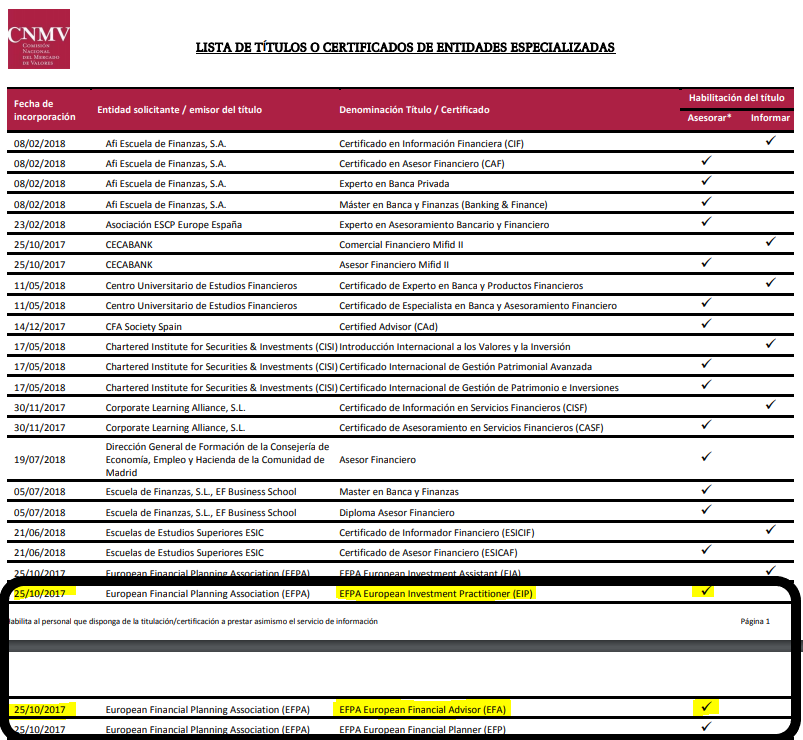
\includegraphics[width=1\textwidth,height=\textheight]{./images/lista_titulos.png}

}

\end{figure}

muchos de los candidatos/as están optando por certificarse com Asesor
Europeo (EFA) primero a través del examen EIP y, una vez que este se
encuentra aprobado, EFPA te ofrece la posibilidad de acceder al EFA
Completo a través de un examen ``parcial'' que sólo supone el 40\%
restante del contenido EFA Completo. Es como descir que el EFA Completo
se compone de,

\begin{itemize}
\item
  \textbf{EIP}: incluye el 60\% del contenido del EFA Completo
\item
  \textbf{EFA Nivel II}: incluye el 40\% restante del contenido del EFA
  Completo.
\end{itemize}

\textbf{¿Qué diferencias hay entre EIP y EFA?}

Como hemos dicho más arriba, una de las acreditaciones más demandadas
actualmente es la nueva certificación EIP, que de una forma resumida,
incluye el siguiente programa de contenidos:

\begin{longtable}[]{@{}clc@{}}
\toprule()
\endhead
Módulo 1 & Instrumentos y mercados financieros & 40,00\% \\
Módulo 2 & Fondos y sociedades de inversión mobiliaria & 10,00\% \\
Módulo 3 & Gestión de carteras & 12,50\% \\
Módulo 4 & Seguros & 7,50\% \\
Módulo 5 & Planes y fondos de pensiones & 5,00\% \\
Módulo 6 & Fiscalidad & 10,00\% \\
Módulo 7 & Cumplimiento normativo y regulador & 7,50\% \\
Módulo 8 & Asesoramiento y planificación financiera & 7,50\% \\
\bottomrule()
\end{longtable}

La siguiente certificación más demanda, y ya consolidada en el mercado,
es la certificación de asesor financiero europeo EFA. Este prestigio
examen incluye el siguiente programa de contenidos:

\begin{longtable}[]{@{}clc@{}}
\toprule()
\endhead
Módulo 1 & Instrumentos y mercados financieros & 25,00\% \\
Módulo 2 & Fondos y sociedades de inversión mobiliaria & 10,00\% \\
Módulo 3 & Gestión de carteras & 17,50\% \\
Módulo 4 & Seguros & 7,50\% \\
Módulo 5 & Pensiones y planificación de jubilación & 5,00\% \\
Módulo 6 & \textbf{Inversión Inmobiliaria} & 5,00\% \\
Módulo 7 & \textbf{Crédito y financiación} & 5,00\% \\
Módulo 8 & Fiscalidad & 10,00\% \\
Módulo 9 & Cumplimiento normativo y regulador & 7,50\% \\
Módulo 10 & Asesoramiento y planificación financiera & 7,50\% \\
\bottomrule()
\end{longtable}

Como se aprecia en los programas EFPA anteriores, el temario del examen
EFA incluye dos módulos más que el temario del examen EIP. Concretamente
los módulos de Inversión Inmobiliaria y, Crédito y financiación.
Asimismo, existen diferencias entre ambos exámenes en los contenidos de
cada uno de los módulos aunque estos tengan el mismo nombre.

Por lo tanto podemos optar por empezar esta formación de forma parcial,
es decir \textbf{podemos acreditarnos como EIP y más tarde como EFA
aprovechando lo común de los contenidos}. De forma que el examen EIP (o
de nivel I):

\begin{longtable}[]{@{}
  >{\centering\arraybackslash}p{(\columnwidth - 6\tabcolsep) * \real{0.2329}}
  >{\raggedright\arraybackslash}p{(\columnwidth - 6\tabcolsep) * \real{0.3014}}
  >{\centering\arraybackslash}p{(\columnwidth - 6\tabcolsep) * \real{0.2329}}
  >{\centering\arraybackslash}p{(\columnwidth - 6\tabcolsep) * \real{0.2329}}@{}}
\toprule()
\begin{minipage}[b]{\linewidth}\centering
\textbf{Módulo}
\end{minipage} & \begin{minipage}[b]{\linewidth}\raggedright
\textbf{Contenidos}
\end{minipage} & \begin{minipage}[b]{\linewidth}\centering
\textbf{Peso}
\end{minipage} & \begin{minipage}[b]{\linewidth}\centering
\textbf{Nº Preguntas}
\end{minipage} \\
\midrule()
\endhead
Módulo 1 & Instrumentos y mercados financieros & 40,00\% & 16 \\
Módulo 2 & Fondos y sociedades de inversión mobiliaria & 10,00\% & 4 \\
Módulo 3 & Gestión de carteras & 12,50\% & 5 \\
Módulo 4 & Seguros & 7,50\% & 3 \\
Módulo 5 & Planes y fondos de pensiones & 5,00\% & 2 \\
Módulo 6 & Fiscalidad & 10,00\% & 4 \\
Módulo 7 & Cumplimiento normativo y regulador & 7,50\% & 3 \\
Módulo 8 & Asesoramiento y planificación financiera & 7,50\% & 3 \\
\textbf{Total}: & & \textbf{100\%} & \textbf{40} \\
\bottomrule()
\end{longtable}

EFPA España ya ha previsto esto y es por ello que ofrece una solución en
la cual el aspirante se acredita primero como EIP y más tarde cabe la
posibilidad de hacer un ``curso puente2 -digamos- que le permitiría al
alumno examinarse de aquellos contenidos que son exclusivos de la
certificación EFPA. Este examen es conocido como examen de''nivel II'' y
es convocado por la Asociación 4 veces al año.

Además, la estructura de cada uno de estos exámenes es diferente como
vemos a continuación:

\textbf{Estructura examen EIP}

El examen EIP consta de 40 preguntas tipo test. Es requisito responder,
al menos, el 70\% de las preguntas del examen correctamente (28
preguntas), para superar satisfactoriamente la prueba. Las respuestas
incorrectas o en blanco no restan puntos. Duración del examen es de 1
hora y 30 minutos.

\textbf{Estructura examen EFA nivel II}

Constará de 2 partes:

La primera, un examen tipo test de 40 preguntas. Para aprobar, el
requisito será el haber respondido bien al menos al 70\% del examen (28
preguntas). Las respuestas incorrectas o en blanco no restan puntos.
Duración de la primera prueba: 1 hora y 30 minutos.

La segunda parte, consistirá en la resolución de ejercicios prácticos
sobre distintos aspectos contemplados en el temario EFA. Duración de la
segunda prueba: 1 hora.

Deben aprobarse ambas partes.

\textbf{Estructura examen EFA completo}

Constará de 2 partes:

La primera, un examen tipo test de 50 preguntas. Para aprobar, el
requisito será el haber respondido bien al menos al 70\% del examen (35
preguntas). Las respuestas incorrectas o en blanco no restan puntos.
Duración de la primera prueba: 1 hora y 30 minutos.

La segunda parte, consistirá en la resolución de ejercicios prácticos
sobre distintos aspectos contemplados en el temario EFA. Duración de la
segunda prueba: 1 hora.

Deben aprobarse ambas partes.

\textbf{¿Necesito algún requisito para acceder a las acreditaciones
profesionales de EFPA}

EFPA exige unos requisitos mínimos y que estos van en función de qué
certificación queramos obtener. A continuación se presenta la
comparativa entre la certificación EIP y EFA:

\textbf{Requisitos examen EIP}

Disponer de titulación completa de estudios secundarios.

Carecer de antecedentes penales por delitos dolosos, no haber sido
objeto de expulsión en colegio o asociación profesional y no haberle
impuesto sanción firme por infracción grave en la CNMV.

Acreditar 6 meses de experiencia en el sector financiero.

Realizar la inscripción al examen, a través de la Web de EFPA,
cumplimentando los datos requeridos, adjuntando CV, la última titulación
académica obtenida y realizar la transferencia de los derechos de examen
para finalizar el proceso (181,50 IVA incluido).

\textbf{Requisitos examen EFA}

Disponer de titulación completa de estudios secundarios.

Se requiere 1 año de experiencia para poder obtener la certificación EFA
o bien, 6 meses, si el candidato ha realizado un curso de preparación en
un centro Acreditado. Una vez, el candidato ha obtenido el APTO, sino
dispone de la experiencia necesaria se le conserva el resultado durante
3 años, o hasta que demuestre haber obtenido la experiencia requerida y
así poder darse de alta en la asociación.

Carecer de antecedentes penales por delitos dolosos, no haber sido
objeto de expulsión en colegio o asociación profesional y no haberle
impuesto sanción firme por infracción grave en la CNMV.

Realizar la inscripción al examen, a través de la Web, cumplimentando
los datos requeridos, adjuntando CV, la última titulación académica
obtenida y realizar la transferencia de los derechos de examen para
finalizar el proceso (225 euros + 21\% IVA).

\part{EJERCICIOS RESUELTOS}

\hypertarget{muxf3dulo-1}{%
\chapter*{Módulo 1}\label{muxf3dulo-1}}
\addcontentsline{toc}{chapter}{Módulo 1}

\markboth{Módulo 1}{Módulo 1}

\begin{enumerate}
\def\labelenumi{\arabic{enumi}.}
\tightlist
\item
  Si en un país, los tipos de interés están al 0.5\%, la inflación al
  4\% y el crecimiento del PIB en el -0.5\%. ¿Qué se espera que haga el
  país para aumentar su producción?
\end{enumerate}

\begin{enumerate}
\def\labelenumi{\alph{enumi})}
\item
  Disminuir tipos de interés.
\item
  Reducir la cantidad de dinero en circulación para que los individuos
  consuman más.
\item
  Devaluar la moneda para incrementar las exportaciones.
\item
  Ninguna de las anteriores.
\end{enumerate}

\begin{tcolorbox}[enhanced jigsaw, opacityback=0, bottomrule=.15mm, colframe=quarto-callout-tip-color-frame, arc=.35mm, leftrule=.75mm, breakable, colback=white, rightrule=.15mm, toprule=.15mm, left=2mm]
\begin{minipage}[t]{5.5mm}
\textcolor{quarto-callout-tip-color}{\faLightbulb}
\end{minipage}%
\begin{minipage}[t]{\textwidth - 5.5mm}

La respuesta \textbf{correcta es la c}.

A pesar de que la devaluación de la moneda puede ser generadora de
inflación, se puede interpretar que el problema más importante de la
economía es el crecimiento económico negativo, y por ello debe tomarse
alguna medida encaminada a fomentar el aumento del PIB, por ello una
devaluación, puede generar aspectos competitivos favorables, en la
medida que pueda fomentar el aumento de las exportaciones y la reducción
de las importaciones, lo que llevaría a aumentar el PIB.

El tipo de interés ya está en unos niveles muy bajos y por ello el
margen de actuación de la Política Monetaria es escaso o nulo.

Reducir la cantidad de dinero en circulación para que los individuos
consuman más, parece absurdo ya que la reducción de dinero produciría un
aumento de los tipos de interés, lo que en principio sería un factor
perjudicial para fomentar el crecimiento económico.

\end{minipage}%
\end{tcolorbox}

\begin{center}\rule{0.5\linewidth}{0.5pt}\end{center}

\hypertarget{muxf3dulo-2}{%
\chapter*{Módulo 2}\label{muxf3dulo-2}}
\addcontentsline{toc}{chapter}{Módulo 2}

\markboth{Módulo 2}{Módulo 2}

\begin{enumerate}
\def\labelenumi{\arabic{enumi}.}
\tightlist
\item
  Si en un país, los tipos de interés están al 0.5\%, la inflación al
  4\% y el crecimiento del PIB en el -0.5\%. ¿Qué se espera que haga el
  país para aumentar su producción?
\end{enumerate}

\begin{enumerate}
\def\labelenumi{\alph{enumi})}
\item
  Disminuir tipos de interés.
\item
  Reducir la cantidad de dinero en circulación para que los individuos
  consuman más.
\item
  Devaluar la moneda para incrementar las exportaciones.
\item
  Ninguna de las anteriores.
\end{enumerate}

\begin{tcolorbox}[enhanced jigsaw, opacityback=0, bottomrule=.15mm, colframe=quarto-callout-tip-color-frame, arc=.35mm, leftrule=.75mm, breakable, colback=white, rightrule=.15mm, toprule=.15mm, left=2mm]
\begin{minipage}[t]{5.5mm}
\textcolor{quarto-callout-tip-color}{\faLightbulb}
\end{minipage}%
\begin{minipage}[t]{\textwidth - 5.5mm}

La respuesta \textbf{correcta es la c}.

A pesar de que la devaluación de la moneda puede ser generadora de
inflación, se puede interpretar que el problema más importante de la
economía es el crecimiento económico negativo, y por ello debe tomarse
alguna medida encaminada a fomentar el aumento del PIB, por ello una
devaluación, puede generar aspectos competitivos favorables, en la
medida que pueda fomentar el aumento de las exportaciones y la reducción
de las importaciones, lo que llevaría a aumentar el PIB.

El tipo de interés ya está en unos niveles muy bajos y por ello el
margen de actuación de la Política Monetaria es escaso o nulo.

Reducir la cantidad de dinero en circulación para que los individuos
consuman más, parece absurdo ya que la reducción de dinero produciría un
aumento de los tipos de interés, lo que en principio sería un factor
perjudicial para fomentar el crecimiento económico.

\end{minipage}%
\end{tcolorbox}

\begin{center}\rule{0.5\linewidth}{0.5pt}\end{center}

\part{EXÁMENES TEST}

\hypertarget{diciembre-2022}{%
\chapter*{Diciembre 2022}\label{diciembre-2022}}
\addcontentsline{toc}{chapter}{Diciembre 2022}

\markboth{Diciembre 2022}{Diciembre 2022}

\begin{enumerate}
\def\labelenumi{\arabic{enumi}.}
\tightlist
\item
  Si en un país, los tipos de interés están al 0.5\%, la inflación al
  4\% y el crecimiento del PIB en el -0.5\%. ¿Qué se espera que haga el
  país para aumentar su producción?
\end{enumerate}

\begin{enumerate}
\def\labelenumi{\alph{enumi})}
\item
  Disminuir tipos de interés.
\item
  Reducir la cantidad de dinero en circulación para que los individuos
  consuman más.
\item
  Devaluar la moneda para incrementar las exportaciones.
\item
  Ninguna de las anteriores.
\end{enumerate}

\begin{tcolorbox}[enhanced jigsaw, opacityback=0, bottomrule=.15mm, colframe=quarto-callout-tip-color-frame, arc=.35mm, leftrule=.75mm, breakable, colback=white, rightrule=.15mm, toprule=.15mm, left=2mm]
\begin{minipage}[t]{5.5mm}
\textcolor{quarto-callout-tip-color}{\faLightbulb}
\end{minipage}%
\begin{minipage}[t]{\textwidth - 5.5mm}

La respuesta \textbf{correcta es la c}.

A pesar de que la devaluación de la moneda puede ser generadora de
inflación, se puede interpretar que el problema más importante de la
economía es el crecimiento económico negativo, y por ello debe tomarse
alguna medida encaminada a fomentar el aumento del PIB, por ello una
devaluación, puede generar aspectos competitivos favorables, en la
medida que pueda fomentar el aumento de las exportaciones y la reducción
de las importaciones, lo que llevaría a aumentar el PIB.

El tipo de interés ya está en unos niveles muy bajos y por ello el
margen de actuación de la Política Monetaria es escaso o nulo.

Reducir la cantidad de dinero en circulación para que los individuos
consuman más, parece absurdo ya que la reducción de dinero produciría un
aumento de los tipos de interés, lo que en principio sería un factor
perjudicial para fomentar el crecimiento económico.

\end{minipage}%
\end{tcolorbox}

\begin{center}\rule{0.5\linewidth}{0.5pt}\end{center}

\hypertarget{septiembre-2022}{%
\chapter*{Septiembre 2022}\label{septiembre-2022}}
\addcontentsline{toc}{chapter}{Septiembre 2022}

\markboth{Septiembre 2022}{Septiembre 2022}

\begin{enumerate}
\def\labelenumi{\arabic{enumi}.}
\tightlist
\item
  Si en un país, los tipos de interés están al 0.5\%, la inflación al
  4\% y el crecimiento del PIB en el -0.5\%. ¿Qué se espera que haga el
  país para aumentar su producción?
\end{enumerate}

\begin{enumerate}
\def\labelenumi{\alph{enumi})}
\item
  Disminuir tipos de interés.
\item
  Reducir la cantidad de dinero en circulación para que los individuos
  consuman más.
\item
  Devaluar la moneda para incrementar las exportaciones.
\item
  Ninguna de las anteriores.
\end{enumerate}

\begin{tcolorbox}[enhanced jigsaw, opacityback=0, bottomrule=.15mm, colframe=quarto-callout-tip-color-frame, arc=.35mm, leftrule=.75mm, breakable, colback=white, rightrule=.15mm, toprule=.15mm, left=2mm]
\begin{minipage}[t]{5.5mm}
\textcolor{quarto-callout-tip-color}{\faLightbulb}
\end{minipage}%
\begin{minipage}[t]{\textwidth - 5.5mm}

La respuesta \textbf{correcta es la c}.

A pesar de que la devaluación de la moneda puede ser generadora de
inflación, se puede interpretar que el problema más importante de la
economía es el crecimiento económico negativo, y por ello debe tomarse
alguna medida encaminada a fomentar el aumento del PIB, por ello una
devaluación, puede generar aspectos competitivos favorables, en la
medida que pueda fomentar el aumento de las exportaciones y la reducción
de las importaciones, lo que llevaría a aumentar el PIB.

El tipo de interés ya está en unos niveles muy bajos y por ello el
margen de actuación de la Política Monetaria es escaso o nulo.

Reducir la cantidad de dinero en circulación para que los individuos
consuman más, parece absurdo ya que la reducción de dinero produciría un
aumento de los tipos de interés, lo que en principio sería un factor
perjudicial para fomentar el crecimiento económico.

\end{minipage}%
\end{tcolorbox}

\begin{center}\rule{0.5\linewidth}{0.5pt}\end{center}

\part{EXÁMENES PRÁCTICA}

\hypertarget{caso-diciembre-2022}{%
\chapter*{Caso diciembre 2022}\label{caso-diciembre-2022}}
\addcontentsline{toc}{chapter}{Caso diciembre 2022}

\markboth{Caso diciembre 2022}{Caso diciembre 2022}

\begin{enumerate}
\def\labelenumi{\arabic{enumi}.}
\tightlist
\item
  Si en un país, los tipos de interés están al 0.5\%, la inflación al
  4\% y el crecimiento del PIB en el -0.5\%. ¿Qué se espera que haga el
  país para aumentar su producción?
\end{enumerate}

\begin{enumerate}
\def\labelenumi{\alph{enumi})}
\item
  Disminuir tipos de interés.
\item
  Reducir la cantidad de dinero en circulación para que los individuos
  consuman más.
\item
  Devaluar la moneda para incrementar las exportaciones.
\item
  Ninguna de las anteriores.
\end{enumerate}

\begin{tcolorbox}[enhanced jigsaw, opacityback=0, bottomrule=.15mm, colframe=quarto-callout-tip-color-frame, arc=.35mm, leftrule=.75mm, breakable, colback=white, rightrule=.15mm, toprule=.15mm, left=2mm]
\begin{minipage}[t]{5.5mm}
\textcolor{quarto-callout-tip-color}{\faLightbulb}
\end{minipage}%
\begin{minipage}[t]{\textwidth - 5.5mm}

La respuesta \textbf{correcta es la c}.

A pesar de que la devaluación de la moneda puede ser generadora de
inflación, se puede interpretar que el problema más importante de la
economía es el crecimiento económico negativo, y por ello debe tomarse
alguna medida encaminada a fomentar el aumento del PIB, por ello una
devaluación, puede generar aspectos competitivos favorables, en la
medida que pueda fomentar el aumento de las exportaciones y la reducción
de las importaciones, lo que llevaría a aumentar el PIB.

El tipo de interés ya está en unos niveles muy bajos y por ello el
margen de actuación de la Política Monetaria es escaso o nulo.

Reducir la cantidad de dinero en circulación para que los individuos
consuman más, parece absurdo ya que la reducción de dinero produciría un
aumento de los tipos de interés, lo que en principio sería un factor
perjudicial para fomentar el crecimiento económico.

\end{minipage}%
\end{tcolorbox}

\begin{center}\rule{0.5\linewidth}{0.5pt}\end{center}

\hypertarget{caso-septiembre-2022}{%
\chapter*{Caso septiembre 2022}\label{caso-septiembre-2022}}
\addcontentsline{toc}{chapter}{Caso septiembre 2022}

\markboth{Caso septiembre 2022}{Caso septiembre 2022}

\begin{enumerate}
\def\labelenumi{\arabic{enumi}.}
\tightlist
\item
  Si en un país, los tipos de interés están al 0.5\%, la inflación al
  4\% y el crecimiento del PIB en el -0.5\%. ¿Qué se espera que haga el
  país para aumentar su producción?
\end{enumerate}

\begin{enumerate}
\def\labelenumi{\alph{enumi})}
\item
  Disminuir tipos de interés.
\item
  Reducir la cantidad de dinero en circulación para que los individuos
  consuman más.
\item
  Devaluar la moneda para incrementar las exportaciones.
\item
  Ninguna de las anteriores.
\end{enumerate}

\begin{tcolorbox}[enhanced jigsaw, opacityback=0, bottomrule=.15mm, colframe=quarto-callout-tip-color-frame, arc=.35mm, leftrule=.75mm, breakable, colback=white, rightrule=.15mm, toprule=.15mm, left=2mm]
\begin{minipage}[t]{5.5mm}
\textcolor{quarto-callout-tip-color}{\faLightbulb}
\end{minipage}%
\begin{minipage}[t]{\textwidth - 5.5mm}

La respuesta \textbf{correcta es la c}.

A pesar de que la devaluación de la moneda puede ser generadora de
inflación, se puede interpretar que el problema más importante de la
economía es el crecimiento económico negativo, y por ello debe tomarse
alguna medida encaminada a fomentar el aumento del PIB, por ello una
devaluación, puede generar aspectos competitivos favorables, en la
medida que pueda fomentar el aumento de las exportaciones y la reducción
de las importaciones, lo que llevaría a aumentar el PIB.

El tipo de interés ya está en unos niveles muy bajos y por ello el
margen de actuación de la Política Monetaria es escaso o nulo.

Reducir la cantidad de dinero en circulación para que los individuos
consuman más, parece absurdo ya que la reducción de dinero produciría un
aumento de los tipos de interés, lo que en principio sería un factor
perjudicial para fomentar el crecimiento económico.

\end{minipage}%
\end{tcolorbox}

\begin{center}\rule{0.5\linewidth}{0.5pt}\end{center}



\end{document}
